% Options for packages loaded elsewhere
\PassOptionsToPackage{unicode}{hyperref}
\PassOptionsToPackage{hyphens}{url}
%
\documentclass[
]{book}
\usepackage{amsmath,amssymb}
\usepackage{lmodern}
\usepackage{ifxetex,ifluatex}
\ifnum 0\ifxetex 1\fi\ifluatex 1\fi=0 % if pdftex
  \usepackage[T1]{fontenc}
  \usepackage[utf8]{inputenc}
  \usepackage{textcomp} % provide euro and other symbols
\else % if luatex or xetex
  \usepackage{unicode-math}
  \defaultfontfeatures{Scale=MatchLowercase}
  \defaultfontfeatures[\rmfamily]{Ligatures=TeX,Scale=1}
\fi
% Use upquote if available, for straight quotes in verbatim environments
\IfFileExists{upquote.sty}{\usepackage{upquote}}{}
\IfFileExists{microtype.sty}{% use microtype if available
  \usepackage[]{microtype}
  \UseMicrotypeSet[protrusion]{basicmath} % disable protrusion for tt fonts
}{}
\makeatletter
\@ifundefined{KOMAClassName}{% if non-KOMA class
  \IfFileExists{parskip.sty}{%
    \usepackage{parskip}
  }{% else
    \setlength{\parindent}{0pt}
    \setlength{\parskip}{6pt plus 2pt minus 1pt}}
}{% if KOMA class
  \KOMAoptions{parskip=half}}
\makeatother
\usepackage{xcolor}
\IfFileExists{xurl.sty}{\usepackage{xurl}}{} % add URL line breaks if available
\IfFileExists{bookmark.sty}{\usepackage{bookmark}}{\usepackage{hyperref}}
\hypersetup{
  pdftitle={Calculus Made EasieR},
  pdfauthor={William Murrah},
  hidelinks,
  pdfcreator={LaTeX via pandoc}}
\urlstyle{same} % disable monospaced font for URLs
\usepackage{color}
\usepackage{fancyvrb}
\newcommand{\VerbBar}{|}
\newcommand{\VERB}{\Verb[commandchars=\\\{\}]}
\DefineVerbatimEnvironment{Highlighting}{Verbatim}{commandchars=\\\{\}}
% Add ',fontsize=\small' for more characters per line
\usepackage{framed}
\definecolor{shadecolor}{RGB}{248,248,248}
\newenvironment{Shaded}{\begin{snugshade}}{\end{snugshade}}
\newcommand{\AlertTok}[1]{\textcolor[rgb]{0.94,0.16,0.16}{#1}}
\newcommand{\AnnotationTok}[1]{\textcolor[rgb]{0.56,0.35,0.01}{\textbf{\textit{#1}}}}
\newcommand{\AttributeTok}[1]{\textcolor[rgb]{0.77,0.63,0.00}{#1}}
\newcommand{\BaseNTok}[1]{\textcolor[rgb]{0.00,0.00,0.81}{#1}}
\newcommand{\BuiltInTok}[1]{#1}
\newcommand{\CharTok}[1]{\textcolor[rgb]{0.31,0.60,0.02}{#1}}
\newcommand{\CommentTok}[1]{\textcolor[rgb]{0.56,0.35,0.01}{\textit{#1}}}
\newcommand{\CommentVarTok}[1]{\textcolor[rgb]{0.56,0.35,0.01}{\textbf{\textit{#1}}}}
\newcommand{\ConstantTok}[1]{\textcolor[rgb]{0.00,0.00,0.00}{#1}}
\newcommand{\ControlFlowTok}[1]{\textcolor[rgb]{0.13,0.29,0.53}{\textbf{#1}}}
\newcommand{\DataTypeTok}[1]{\textcolor[rgb]{0.13,0.29,0.53}{#1}}
\newcommand{\DecValTok}[1]{\textcolor[rgb]{0.00,0.00,0.81}{#1}}
\newcommand{\DocumentationTok}[1]{\textcolor[rgb]{0.56,0.35,0.01}{\textbf{\textit{#1}}}}
\newcommand{\ErrorTok}[1]{\textcolor[rgb]{0.64,0.00,0.00}{\textbf{#1}}}
\newcommand{\ExtensionTok}[1]{#1}
\newcommand{\FloatTok}[1]{\textcolor[rgb]{0.00,0.00,0.81}{#1}}
\newcommand{\FunctionTok}[1]{\textcolor[rgb]{0.00,0.00,0.00}{#1}}
\newcommand{\ImportTok}[1]{#1}
\newcommand{\InformationTok}[1]{\textcolor[rgb]{0.56,0.35,0.01}{\textbf{\textit{#1}}}}
\newcommand{\KeywordTok}[1]{\textcolor[rgb]{0.13,0.29,0.53}{\textbf{#1}}}
\newcommand{\NormalTok}[1]{#1}
\newcommand{\OperatorTok}[1]{\textcolor[rgb]{0.81,0.36,0.00}{\textbf{#1}}}
\newcommand{\OtherTok}[1]{\textcolor[rgb]{0.56,0.35,0.01}{#1}}
\newcommand{\PreprocessorTok}[1]{\textcolor[rgb]{0.56,0.35,0.01}{\textit{#1}}}
\newcommand{\RegionMarkerTok}[1]{#1}
\newcommand{\SpecialCharTok}[1]{\textcolor[rgb]{0.00,0.00,0.00}{#1}}
\newcommand{\SpecialStringTok}[1]{\textcolor[rgb]{0.31,0.60,0.02}{#1}}
\newcommand{\StringTok}[1]{\textcolor[rgb]{0.31,0.60,0.02}{#1}}
\newcommand{\VariableTok}[1]{\textcolor[rgb]{0.00,0.00,0.00}{#1}}
\newcommand{\VerbatimStringTok}[1]{\textcolor[rgb]{0.31,0.60,0.02}{#1}}
\newcommand{\WarningTok}[1]{\textcolor[rgb]{0.56,0.35,0.01}{\textbf{\textit{#1}}}}
\usepackage{longtable,booktabs,array}
\usepackage{calc} % for calculating minipage widths
% Correct order of tables after \paragraph or \subparagraph
\usepackage{etoolbox}
\makeatletter
\patchcmd\longtable{\par}{\if@noskipsec\mbox{}\fi\par}{}{}
\makeatother
% Allow footnotes in longtable head/foot
\IfFileExists{footnotehyper.sty}{\usepackage{footnotehyper}}{\usepackage{footnote}}
\makesavenoteenv{longtable}
\usepackage{graphicx}
\makeatletter
\def\maxwidth{\ifdim\Gin@nat@width>\linewidth\linewidth\else\Gin@nat@width\fi}
\def\maxheight{\ifdim\Gin@nat@height>\textheight\textheight\else\Gin@nat@height\fi}
\makeatother
% Scale images if necessary, so that they will not overflow the page
% margins by default, and it is still possible to overwrite the defaults
% using explicit options in \includegraphics[width, height, ...]{}
\setkeys{Gin}{width=\maxwidth,height=\maxheight,keepaspectratio}
% Set default figure placement to htbp
\makeatletter
\def\fps@figure{htbp}
\makeatother
\setlength{\emergencystretch}{3em} % prevent overfull lines
\providecommand{\tightlist}{%
  \setlength{\itemsep}{0pt}\setlength{\parskip}{0pt}}
\setcounter{secnumdepth}{5}
\usepackage{booktabs}
\usepackage{booktabs}
\usepackage{longtable}
\usepackage{array}
\usepackage{multirow}
\usepackage{wrapfig}
\usepackage{float}
\usepackage{colortbl}
\usepackage{pdflscape}
\usepackage{tabu}
\usepackage{threeparttable}
\usepackage{threeparttablex}
\usepackage[normalem]{ulem}
\usepackage{makecell}
\usepackage{xcolor}
\ifluatex
  \usepackage{selnolig}  % disable illegal ligatures
\fi
\usepackage[]{natbib}
\bibliographystyle{apalike}

\title{Calculus Made EasieR}
\author{William Murrah}
\date{2021-08-08}

\begin{document}
\maketitle

{
\setcounter{tocdepth}{1}
\tableofcontents
}
\hypertarget{preface}{%
\chapter*{Preface}\label{preface}}
\addcontentsline{toc}{chapter}{Preface}

This is a collection of notes I generated while using R to learn calculus for statistics in general and nonlinear modeling specifically.
The notes are based multiple sources including a classic book by \citet{thompson1998calculus}, and a great textbook focusing on calculus and probability in the life sciences\citep{adler2012modeling}.

\hypertarget{intro}{%
\chapter{Introduction}\label{intro}}

\hypertarget{algebra-and-calculus-basics}{%
\section{Algebra and Calculus Basics}\label{algebra-and-calculus-basics}}

\hypertarget{exponentials-and-logarithms}{%
\subsection{Exponentials and Logarithms}\label{exponentials-and-logarithms}}

An exponential is represented as \(e^x\) or exp(\(x\)), with \(e\) being the constant 2.718\ldots.
Some things to know about exponentials, and how to generate them in are include \citep{bolker2008ecological}:

\(\text{exp}(1) = e = 2.718282\),

\begin{Shaded}
\begin{Highlighting}[]
\FunctionTok{exp}\NormalTok{(}\DecValTok{1}\NormalTok{)}
\end{Highlighting}
\end{Shaded}

\begin{verbatim}
## [1] 2.718282
\end{verbatim}

\(\text{exp}(0) = 1\),

\begin{Shaded}
\begin{Highlighting}[]
\FunctionTok{exp}\NormalTok{(}\DecValTok{0}\NormalTok{)}
\end{Highlighting}
\end{Shaded}

\begin{verbatim}
## [1] 1
\end{verbatim}

\(\text{exp}(-\infty) = 0\),

\begin{Shaded}
\begin{Highlighting}[]
\FunctionTok{exp}\NormalTok{(}\SpecialCharTok{{-}}\ConstantTok{Inf}\NormalTok{)}
\end{Highlighting}
\end{Shaded}

\begin{verbatim}
## [1] 0
\end{verbatim}

and \(\text{exp}(\infty) = \infty\),

\begin{Shaded}
\begin{Highlighting}[]
\FunctionTok{exp}\NormalTok{(}\ConstantTok{Inf}\NormalTok{)}
\end{Highlighting}
\end{Shaded}

\begin{verbatim}
## [1] Inf
\end{verbatim}

Logarithms can have

\hypertarget{functions}{%
\chapter{Functions}\label{functions}}

Two functions, \(f(x)\) and \(g(x)\) are below:

\[
f(x) = 4 + x - x^2 \label{eq:f} 
\]

\[
g(x) = 2x \label{eq:g}
\]

\begin{Shaded}
\begin{Highlighting}[]
\NormalTok{f }\OtherTok{\textless{}{-}} \ControlFlowTok{function}\NormalTok{(x) }\DecValTok{4} \SpecialCharTok{+}\NormalTok{ x }\SpecialCharTok{{-}}\NormalTok{ x}\SpecialCharTok{\^{}}\DecValTok{2}
\NormalTok{g }\OtherTok{\textless{}{-}} \ControlFlowTok{function}\NormalTok{(x) }\DecValTok{2}\SpecialCharTok{*}\NormalTok{x}
\end{Highlighting}
\end{Shaded}

\hypertarget{composition-of-functions}{%
\subsection{Composition of Functions}\label{composition-of-functions}}

\[
(f \circ g)(x) = f(g(x)) \label{eq:comp}
\]

\begin{Shaded}
\begin{Highlighting}[]
\NormalTok{x }\OtherTok{\textless{}{-}} \FunctionTok{seq}\NormalTok{(}\DecValTok{0}\NormalTok{, }\DecValTok{3}\NormalTok{, .}\DecValTok{5}\NormalTok{)}
\NormalTok{fx }\OtherTok{\textless{}{-}} \FunctionTok{f}\NormalTok{(x)}
\NormalTok{gx }\OtherTok{\textless{}{-}} \FunctionTok{g}\NormalTok{(x)}
\NormalTok{f\_gx }\OtherTok{\textless{}{-}} \FunctionTok{f}\NormalTok{(x) }\SpecialCharTok{+} \FunctionTok{g}\NormalTok{(x)   }\CommentTok{\# (f + g)(x) adding functions}
\NormalTok{f.gx }\OtherTok{\textless{}{-}} \FunctionTok{f}\NormalTok{(x) }\SpecialCharTok{*} \FunctionTok{g}\NormalTok{(x)   }\CommentTok{\# (f * g)(x) multiplying functions}
\NormalTok{fgx }\OtherTok{\textless{}{-}} \FunctionTok{f}\NormalTok{(}\FunctionTok{g}\NormalTok{(x))        }\CommentTok{\# (f o g)(x) composition of functions}

\NormalTok{modelsummary}\SpecialCharTok{::}\FunctionTok{datasummary\_df}\NormalTok{(}\FunctionTok{data.frame}\NormalTok{(x, fx, gx, f\_gx, f.gx, fgx), }\AttributeTok{title =} \StringTok{"Combining Functions"}\NormalTok{)}
\end{Highlighting}
\end{Shaded}

\begin{table}

\caption{\label{tab:tabfg}Combining Functions}
\centering
\begin{tabular}[t]{llllll}
\toprule
x & fx & gx & f\_gx & f.gx & fgx\\
\midrule
0.00 & 4.00 & 0.00 & 4.00 & 0.00 & 4.00\\
0.50 & 4.25 & 1.00 & 5.25 & 4.25 & 4.00\\
1.00 & 4.00 & 2.00 & 6.00 & 8.00 & 2.00\\
1.50 & 3.25 & 3.00 & 6.25 & 9.75 & -2.00\\
2.00 & 2.00 & 4.00 & 6.00 & 8.00 & -8.00\\
2.50 & 0.25 & 5.00 & 5.25 & 1.25 & -16.00\\
3.00 & -2.00 & 6.00 & 4.00 & -12.00 & -26.00\\
\bottomrule
\end{tabular}
\end{table}

\begin{Shaded}
\begin{Highlighting}[]
\NormalTok{x }\OtherTok{\textless{}{-}} \FunctionTok{seq}\NormalTok{(}\DecValTok{0}\NormalTok{, }\DecValTok{3}\NormalTok{, .}\DecValTok{001}\NormalTok{)}
\FunctionTok{plot}\NormalTok{(}\FunctionTok{f}\NormalTok{(x) }\SpecialCharTok{\textasciitilde{}}\NormalTok{ x, }\AttributeTok{type =} \StringTok{"l"}\NormalTok{, }\AttributeTok{ylim =} \FunctionTok{c}\NormalTok{(}\DecValTok{0}\NormalTok{, }\DecValTok{10}\NormalTok{), }\AttributeTok{ylab =} \StringTok{""}\NormalTok{)}
\FunctionTok{text}\NormalTok{(}\FloatTok{2.8}\NormalTok{, .}\DecValTok{3}\NormalTok{, }\AttributeTok{labels =} \StringTok{"f(x)"}\NormalTok{)}
\FunctionTok{lines}\NormalTok{(}\FunctionTok{g}\NormalTok{(x) }\SpecialCharTok{\textasciitilde{}}\NormalTok{ x, }\AttributeTok{col =} \StringTok{"grey"}\NormalTok{)}
\FunctionTok{text}\NormalTok{(}\FloatTok{2.6}\NormalTok{, }\FloatTok{6.1}\NormalTok{, }\StringTok{"g(x)"}\NormalTok{, }\AttributeTok{col =} \StringTok{"grey"}\NormalTok{)}
\FunctionTok{lines}\NormalTok{(}\FunctionTok{f}\NormalTok{(x) }\SpecialCharTok{+} \FunctionTok{g}\NormalTok{(x) }\SpecialCharTok{\textasciitilde{}}\NormalTok{ x, }\AttributeTok{col =} \StringTok{"red"}\NormalTok{)}
\FunctionTok{text}\NormalTok{(}\FloatTok{2.8}\NormalTok{, }\FloatTok{3.6}\NormalTok{, }\StringTok{"f(x) + g(x)"}\NormalTok{, }\AttributeTok{col =} \StringTok{"red"}\NormalTok{)}
\FunctionTok{lines}\NormalTok{(}\FunctionTok{f}\NormalTok{(x) }\SpecialCharTok{*} \FunctionTok{g}\NormalTok{(x) }\SpecialCharTok{\textasciitilde{}}\NormalTok{ x, }\AttributeTok{col =} \StringTok{"blue"}\NormalTok{)}
\FunctionTok{text}\NormalTok{(}\FloatTok{2.3}\NormalTok{, }\DecValTok{8}\NormalTok{, }\StringTok{"f(x) * g(x)"}\NormalTok{, }\AttributeTok{col =} \StringTok{"blue"}\NormalTok{)}
\FunctionTok{lines}\NormalTok{(}\FunctionTok{f}\NormalTok{(}\FunctionTok{g}\NormalTok{(x)) }\SpecialCharTok{\textasciitilde{}}\NormalTok{ x, }\AttributeTok{col =} \StringTok{"green"}\NormalTok{)}
\FunctionTok{text}\NormalTok{(}\FloatTok{1.5}\NormalTok{, .}\DecValTok{3}\NormalTok{, }\StringTok{"f(g(x))"}\NormalTok{, }\AttributeTok{col =} \StringTok{"green"}\NormalTok{)}
\end{Highlighting}
\end{Shaded}

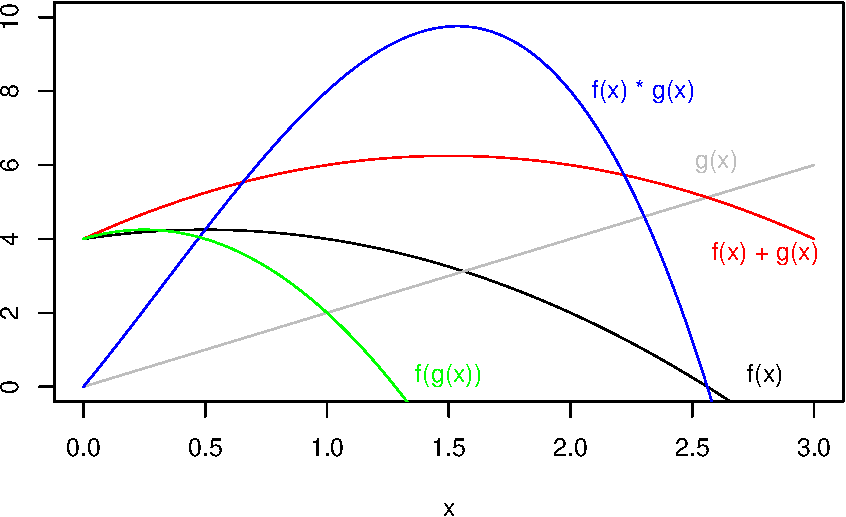
\includegraphics{CalculusMadeEasieR_files/figure-latex/unnamed-chunk-6-1.pdf}

Note that when \(x\) is zero, \(f(x)\) is 4, and \(g(x)\) is zero.
So it makes sense that \(g(x)\) starts at 0 on the y-axis.
It also make sense that \((f * g)\) starts at zero on the y-axis, because any value of \(f(x)\) will be multiplied by zero, which will result in zero.
It is also intuitive that both \(f(x)\) and \(f(x) + g(x)\) start at 4 on the y axis, because \(f(x)\) is 4 when \(x\) is zero (\(f(x) = 0\)), and adding zero to this does not change this value (\(f(x) + g(x) = (4 + 0) = 4\), when \(x=0\)).

\hypertarget{finding-inverse-functions}{%
\subsection{1.2.4 Finding Inverse Functions}\label{finding-inverse-functions}}

\hypertarget{methods}{%
\chapter{Methods}\label{methods}}

We describe our methods in this chapter.

\hypertarget{applications}{%
\chapter{Applications}\label{applications}}

Some \emph{significant} applications are demonstrated in this chapter.

\hypertarget{example-one}{%
\section{Example one}\label{example-one}}

\hypertarget{example-two}{%
\section{Example two}\label{example-two}}

\hypertarget{final-words}{%
\chapter{Final Words}\label{final-words}}

We have finished a nice book.

  \bibliography{book.bib}

\end{document}
